
%(BEGIN_QUESTION)
% Copyright 2006, Tony R. Kuphaldt, released under the Creative Commons Attribution License (v 1.0)
% This means you may do almost anything with this work of mine, so long as you give me proper credit

Shown here is a simple flow control system for distributing water from an irrigation reservoir to a crop field at a controlled flow rate.  The flowmeter is ranged from 0 to 300 gallons per minute:

$$\includegraphics[width=15.5cm]{i01584x01.eps}$$

The flow-recording controller (FRC) is a proportional-only unit with the following algorithm:

$$m = K_p (\hbox{SP} - \hbox{PV}) + 50\hbox{\%}$$

\noindent
Where,

$m$ = Manipulated variable (output)

$K_p$ = Controller gain

SP = Setpoint

PV = Process Variable (water flow)

\vskip 10pt

One day the controller is found to be working perfectly: the setpoint is set to 180 GPM, and the process variable reads exactly the same: 180 GPM.  The controller's output is seen to be 50\% in this condition.  Then, the operator adjusts the setpoint to a new flow rate: 250 GPM.  As expected, the controller's output automatically increases and the valve opens up to allow more flow through the pipe.  As the flow rate approaches the new setpoint of 250 GPM, the valve begins to close off.  This makes the flow rate approach setpoint slower and slower, like a capacitor slowly charging to a new voltage value over time.  However, the operator notices something unexpected: the flow rate never makes it all the way to the new setpoint value of 250 GPM.  Instead, it stabilizes at about 239 GPM and does not increase beyond that.

Confused as to why the controller does not reach the new setpoint of 250 GPM like it did the old setpoint of 180 GPM, the operator calls an instrument technician to investigate.  ``What is wrong with this controller?'' the operator asks the technician.  ``It stops increasing the flow rate shy of its new setpoint.''  After a moment of investigation, the technician notices that this is a proportional-only controller.  Seeing this, the technician just smiles and proceeds to explain to the operator why the controller {\it never will} reach the new setpoint like it did at 180 GPM.  For that matter, it cannot perfectly reach any setpoint less than 180 GPM either!  If it perfectly attained setpoint at 180 GPM, then that is the {\it only} setpoint value it will.

Explain, in your own words, why this is true.

\underbar{file i01584}
%(END_QUESTION)





%(BEGIN_ANSWER)

I will answer this question with another question: imagine if the controller actually {\it did} attain the new setpoint value of 250 GPM.  If it did, what would the valve position be in this condition of equilibrium where both SP and PV are equal to 250 GPM?  Now, compare this with the valve position when both SP and PV were equal to 180 GPM.  Do you see now why PV = SP = 250 GPM is impossible?

\vskip 10pt

Challenge question: what effect does gain ($K_p$) have on the controller's inability to attain setpoint values other than 180 GPM?

%(END_ANSWER)





%(BEGIN_NOTES)

The greater the gain, the less offset.  However, too much gain will result in oscillation.

%INDEX% Control, proportional: proportional-only offset
%INDEX% Process: irrigation water flow

%(END_NOTES)


